\documentclass[presentation,english,usenames,dvipsnames]{beamer}
\usepackage[utf8]{inputenc}
\usepackage{babel}
\usepackage{graphicx}
\usepackage{longtable}
\usepackage{float}
\usepackage{wrapfig}
\usepackage{soul}
\usepackage{textcomp}
\usepackage{marvosym}
\usepackage{wasysym}
\usepackage{latexsym}
\usepackage{amssymb}
\usepackage{hyperref}
\tolerance=1000
\usepackage{listings}
\usepackage[iso]{isodate}
\usepackage{pgfgantt}
\usepackage[font=scriptsize, skip=0pt]{caption}
\usepackage[font=scriptsize, skip=0pt]{subcaption}
\usepackage{pgfplots, pgfplotstable}
\pgfplotsset{compat=1.14}
\usetikzlibrary{fit}

\title[Peer-to-Peer Incentives]{Incentivizing Peers to contribute in a
Low-Latency Name-Lookup Service}
\author{Marc Lehmann}
\subtitle{Initial Master Talk, 2nd try}
\date{\today}


\usetheme{Comsys}
% Adjust the title font size, because my title spans 3 lines otherwise.
\setbeamerfont{title}{size*={16}{26.4},series=\bfseries}

\begin{document}

\setbeamertemplate{footline}[empty]
\begin{frame}
  \titlepage
\end{frame}

\setbeamertemplate{footline}[comsys]

\begin{frame}{Motivation}
  \begin{itemize}
    \item Name-mapping service important to facilitate communication
    \begin{itemize}
      \item names to IPs (DNS)
      \item people to devices (instant messaging)
    \end{itemize}
    \item Privacy concerns in centralized systems
    \begin{itemize}
      \item Server gets a lot of information about whom a user communicates with
      \item Can build user profiles
      \item Can become target for others who want to build profiles
    \end{itemize}
    \item Spread requests to many different nodes in a DHT
    \item Requires lots of nodes \rightarrow users need to participate
          themselves
  \end{itemize}
\end{frame}

\begin{frame}{Encouraging peers to contribute}
  \begin{itemize}
    \item Only leverage: users want good service
    \item Give bad peers bad service
    \item Track how good peers are via a reputation system
    \item Existing solutions to track reputation insufficient
    \begin{itemize}
      \item Require central authority
      \item Or introduce additional latency (using another DHT)
    \end{itemize}
    \item Solution: Track reputation in small subsets of peers (query groups)
  \end{itemize}
\end{frame}

\begin{frame}{Query Groups (Chord)}
  \begin{minipage}{0.5\textwidth}
    \begin{itemize}
      \item Using Chord to illustrate
      \item Need to be able to reach peers in finger table
      \item Need to share a query group with each of these peers
      \item (Not necessarily the same for all)
    \end{itemize}
  \end{minipage}% This comment is necessary to remove any space between the minipages
  \begin{minipage}{0.5\textwidth}
    \begin{figure}
      \centering
      \begin{tikzpicture}
        \begin{scope}[every node/.style={
          circle,
          fill=black,
          inner sep=0pt,
          minimum size=5pt
          }]
          \node[minimum size=8pt] (A) at (90:2) {};
          \node[red] (B) at (30:2) {};
          \node[blue] (C) at (330:2) {};
          \node[violet] (D) at (270:2) {};
          \node[OliveGreen] (E) at (210:2) {};
          \node (F) at (150:2) {};
        \end{scope}

        \draw (B) -- (C)[draw=none] node[midway, sloped] {\ldots};
        \draw (C) -- (D)[draw=none] node[midway, sloped] {\ldots};
        \draw (D) -- (E)[draw=none] node[midway, sloped] {\ldots};
        \draw (E) -- (F)[draw=none] node[midway, sloped] {\ldots};
        \draw (F) -- (A)[draw=none] node[midway, sloped] {\ldots};

        \draw[->] (A) -- (B);
        \draw[->] (A) -- (C);
        \draw[->] (A) -- (D);
        \draw[->] (A) -- (E);

        \begin{pgfonlayer}{background}
          \begin{scope}[every node/.style={
            ellipse,
            draw=black,
            thick,
            inner sep=0pt,
            inner xsep=0pt,
            inner ysep=0pt,
            opacity=0.5
          }]
            \invisible{
              \node[fit=(A)(B), fill=red!30, rotate=-30] {};
            }
            \invisible{
              \node[fit=(A)(C)(D), fill=violet!30, rotate=18, xshift=-15pt] {};
            }
            \invisible{
              \node[fit=(A)(E), fill=OliveGreen!30, rotate=-30,
                    inner xsep=-15pt] {};
            }
          \end{scope}
        \end{pgfonlayer}
      \end{tikzpicture}
    \end{figure}
  \end{minipage}
\end{frame}

\begin{frame}{Query Groups (Chord)}
  \begin{minipage}{0.5\textwidth}
    \begin{itemize}
      \item \visible<1->{Join query group with red peer}
      \item \visible<2->{Join query group with blue peer}
      \item \visible<2->{Purple peer is also in that group}
      \item \visible<3->{Join query group with green peer}
    \end{itemize}
  \end{minipage}% This comment is necessary to remove any space between the minipages
  \begin{minipage}{0.5\textwidth}
    \begin{figure}
      \centering
      \begin{tikzpicture}
        \begin{scope}[every node/.style={
          circle,
          fill=black,
          inner sep=0pt,
          minimum size=5pt
          }]
          \node[minimum size=8pt] (A) at (90:2) {};
          \node[red] (B) at (30:2) {};
          \node[blue] (C) at (330:2) {};
          \node[violet] (D) at (270:2) {};
          \node[OliveGreen] (E) at (210:2) {};
          \node (F) at (150:2) {};
        \end{scope}

        \draw (B) -- (C)[draw=none] node[midway, sloped] {\ldots};
        \draw (C) -- (D)[draw=none] node[midway, sloped] {\ldots};
        \draw (D) -- (E)[draw=none] node[midway, sloped] {\ldots};
        \draw (E) -- (F)[draw=none] node[midway, sloped] {\ldots};
        \draw (F) -- (A)[draw=none] node[midway, sloped] {\ldots};

        \draw[->] (A) -- (B);
        \draw[->] (A) -- (C);
        \draw[->] (A) -- (D);
        \draw[->] (A) -- (E);

        \begin{pgfonlayer}{background}
          \begin{scope}[every node/.style={
            ellipse,
            draw=black,
            thick,
            inner sep=0pt,
            inner xsep=0pt,
            inner ysep=0pt,
            opacity=0.5
          }]
            \visible<1->{
              \node[fit=(A)(B), fill=red!30, rotate=-30] {};
            }
            \visible<2->{
              \node[fit=(A)(C)(D), fill=violet!30, rotate=18, xshift=-15pt] {};
            }
            \visible<3->{
              \node[fit=(A)(E), fill=OliveGreen!30, rotate=-30,
                    inner xsep=-15pt] {};
            }
          \end{scope}
        \end{pgfonlayer}
      \end{tikzpicture}
    \end{figure}
  \end{minipage}
\end{frame}

\begin{frame}{Goal of the Thesis}
  \begin{itemize}
    \item Does such an incentive system lead to a useful system?
    \item Simulate a network of peers with discrete event simulation
    \item Vary parameters of the system
    \item Observe performance characteristics during different runs
    \begin{itemize}
      \item Query response times
      \item Unanswered queries
      \item Distribution of reputation
      \item Query group connectedness
    \end{itemize}
  \end{itemize}
\end{frame}

\begin{frame}{Simulation - Example}
  \begin{itemize}
    \item Existing prototype in SimPy, many simplifications
    \item Compare 2 runs
    \begin{itemize}
      \item Peers respond to every query
      \item Peers only respond if they profit from it
      \begin{itemize}
        \item Optimal service is granted to peers with at least 10 reputation
              points
        \item Peers only respond if they have less than 15 reputation points
      \end{itemize}
    \end{itemize}
    \item 64 peers
    \item Every peer generates one random request per time unit
  \end{itemize}
\end{frame}

\begin{frame}{Simulation - Example}
  \begin{table}
    \centering
    \begin{tabular}{|l|l|l|}
      \hline
      & good peers & selfish peers \\
      \hline
      successful & 2841 (92.8\%) & 2868 (69.4\%) \\
      \hline
      timed out & 217 (7.1\%) & 1236 (29.9\%) \\
      \hline
      unsuccessful & 1 (<0.1\%) & 10 (0.2\%) \\
      \hline
      ultimately timed out & 3 (0.1\%)  & 21 (0.5\%) \\
      \hline
      ultimately unsuccessful & 0 & 0 \\
      \hline
      total & 3062 & 4135 \\
      \hline
    \end{tabular}
    \caption*{Responses arriving during simulated time 50-100}
  \end{table}
  \begin{itemize}
    \item Selfish peers let queries time out
    \item Also means more traffic in total (retries)
    \item Good peer timeouts: unexpected penalty during a recursive query
  \end{itemize}
\end{frame}

\begin{frame}{Simulation - Example}
  \begin{figure}
    \centering
    \begin{subfigure}{.5\textwidth}
      \begin{tikzpicture}[font=\tiny]
        \begin{axis}[
          width=\textwidth,
          height=4cm,
          ybar,
          ymin=0,
          xlabel=response time,
          ylabel=\# peers,
          nodes near coords={
            \pgfmathparse{int(round(\pgfplotspointmetatransformed))}
            \ifnum \pgfmathresult < 5
              \pgfmathprintnumber{\pgfplotspointmeta}
            \fi},
          every node near coord/.append style={
            anchor=south,
            xshift=2pt
          }
        ]
          \addplot +[hist={bins=24, data min=0, data max=24}]
            table[y index=0]{good_response_times.csv};
        \end{axis}
      \end{tikzpicture}
      \caption*{Good peers}
    \end{subfigure}% This comment is necessary to remove any space between the subfigures
    \begin{subfigure}{.5\textwidth}
      \begin{tikzpicture}[font=\tiny]
        \begin{axis}[
          width=\textwidth,
          height=4cm,
          ybar,
          ymin=0,
          xlabel=response time,
          ylabel=\# peers,
          nodes near coords={
            \pgfmathparse{int(round(\pgfplotspointmetatransformed))}
            \ifnum \pgfmathresult < 5
              \pgfmathprintnumber{\pgfplotspointmeta}
            \fi},
          every node near coord/.append style={
            anchor=south,
            xshift=1.4pt
          }
        ]
          \addplot +[hist={bins=37, data min=0, data max=37}]
            table[y index=0]{selfish_response_times.csv};
        \end{axis}
      \end{tikzpicture}
      \caption*{Selfish peers}
    \end{subfigure}
    \caption*{Response times during simulated time 50-100}
  \end{figure}
  \begin{itemize}
    \item Up to 10 time units penalty delay
    \item Good: Many responses at maximum delay, many peers with no reputation
          (artefact of simulation)
    \item Selfish: somtimes multiple attempts necessary (timeouts)
  \end{itemize}
\end{frame}

\begin{frame}{Simulation - Example}
  \begin{figure}
    \centering
    \begin{subfigure}{.5\textwidth}
      \begin{tikzpicture}[font=\tiny]
        \begin{axis}[
          width=\textwidth,
          height=4cm,
          ybar,
          ymin=0,
          xlabel=reputation,
          ylabel=\# peers,
          xtick distance=25
        ]
          \addplot +[hist={bins=25, data min=0, data max=125}]
            table[y index=1]{good_query_group.csv};
        \end{axis}
      \end{tikzpicture}
      \caption*{Good peers}
    \end{subfigure}% This comment is necessary to remove any space between the subfigures
    \begin{subfigure}{.5\textwidth}
      \begin{tikzpicture}[font=\tiny]
        \begin{axis}[
          width=\textwidth,
          height=4cm,
          ybar,
          ymin=0,
          xlabel=reputation,
          ylabel=\# peers,
          xtick distance=25
        ]
          \addplot +[hist={bins=25, data min=0, data max=125}]
            table[y index=1]{selfish_query_group.csv};
        \end{axis}
      \end{tikzpicture}
      \caption*{Selfish peers}
    \end{subfigure}
    \caption*{Reputation distribution at simulation time 100 in a particular
              query group}
  \end{figure}
  \begin{itemize}
    \item Good: Many peers with little reputation, because peers chosen in same
          order (artefact of simulation)
    \item Peers that get chosen a lot have much greater reputation
    \item Selfish: Peers don't get much more than 15 reputation
  \end{itemize}
\end{frame}

\begin{frame}{Simplification - Example}
  \begin{itemize}
    \item Currently, query groups are just sets
    \item Peers just add themselves or others
    \item Always iterate in the same order \rightarrow uneven reputation
          distribution
    \item Each peer needs to maintain group information locally
    \item Join by being invited
    \item Observe how query groups form
    \begin{itemize}
      \item Peers can decline invites if there's no benefit for them
      \item Peers can leave query groups if they get too full
      \item Do peers have trouble getting connectivity?
    \end{itemize}
  \end{itemize}
\end{frame}

\begin{frame}{Summary}
  \begin{itemize}
    \item Get peers to contribute to a name-lookup service
    \item Proposed a reputation tracking system that's supposed to handle the
          low-latency requirement
    \item Implement and evaluate via discrete event simulation
    \item Optional: analytical, game-theoretic solution
  \end{itemize}
\end{frame}

\begin{frame}
\end{frame}

\begin{frame}{Query Groups (Kademlia/P-Grid)}
  \begin{itemize}
    \item View keys as bitstring
    \item Peers have a prefix (bitstring): store keys that start with that
          prefix
    \item Peers are in contact with others with the same prefix (replication)
    \item Other prefixes: know other peers closer to them
  \end{itemize}
  \begin{figure}
    \centering
    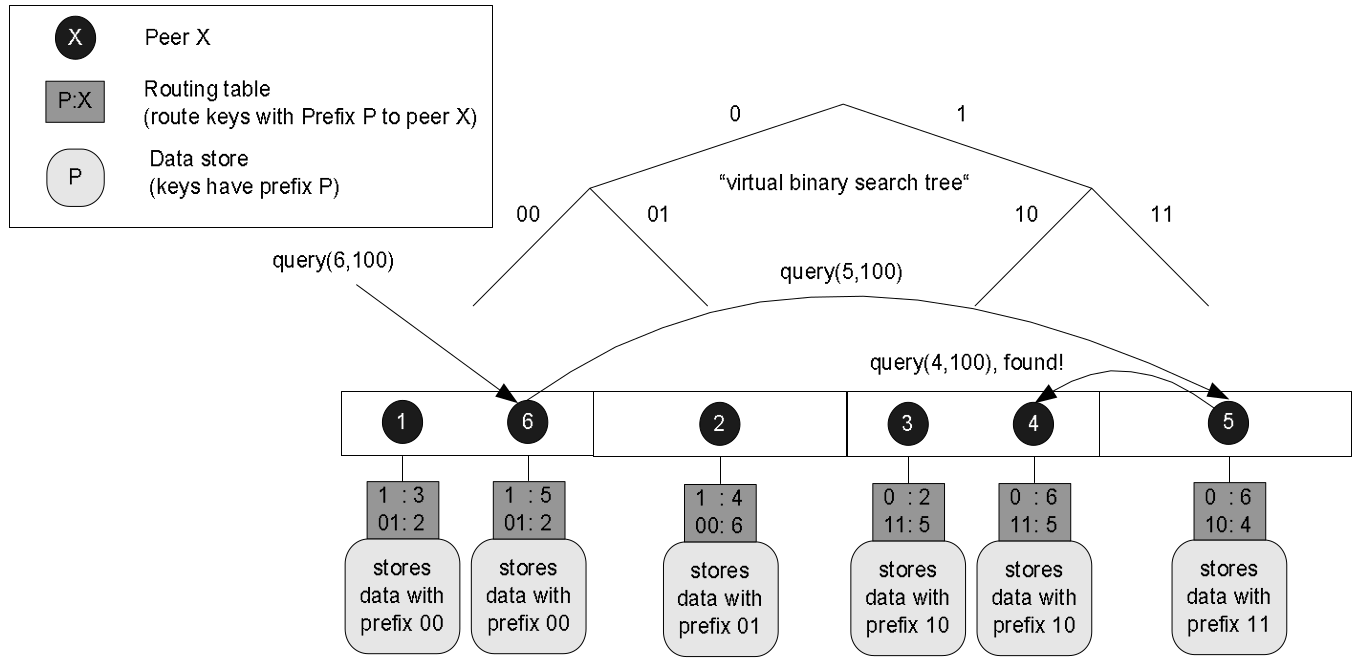
\includegraphics[width=0.5\textwidth]{p-grid}
    \caption*{\tiny From \emph{P-Grid: A Self-organizing Structured P2P System}}
  \end{figure}
\end{frame}

\begin{frame}{Query Groups (Kademlia/P-Grid)}
  \begin{itemize}
    \item Dashed: Same prefix, replication (sync groups)
    \item Solid: Query groups
  \end{itemize}
  \begin{figure}
    \centering
    \begin{tikzpicture}
      \begin{scope}[every node/.style={draw}]
        \node[color=red] (A) at (0:2) {P: 001};
        \node[color=blue] (B) at (45:2) {P: 001};
        \node[color=red] (C) at (90:2) {P: 001};
        \node[color=blue] (D) at (135:2) {P: 010};
        \node[color=OliveGreen] (E) at (180:2) {P: 010};
        \node[color=blue] (F) at (225:2) {P: 101};
        \node[color=red] (G) at (270:2) {P: 101};
        \node[color=OliveGreen] (H) at (315:2) {P: 101};
      \end{scope}

      \path (A) edge[thick,dashed,bend right=15] (B);
      \path (B) edge[thick,dashed,bend right=15] (C);
      \path (A) edge[thick,dashed,bend left=15] (C);
      \path (D) edge[thick,dashed,bend right=15] (E);
      \path (F) edge[thick,dashed,bend right=15] (G);
      \path (G) edge[thick,dashed,bend right=15] (H);
      \path (F) edge[thick,dashed,bend left=15] (H);
      \path (A) edge[thick,color=red,bend left=20] (C);
      \path (C) edge[thick,color=red] (G);
      \path (A) edge[thick,color=red,bend right=15] (G);
      \path (B) edge[thick,color=blue] (D);
      \path (D) edge[thick,color=blue,bend left=15] (F);
      \path (B) edge[thick,color=blue] (F);
      \path (E) edge[thick,color=OliveGreen] (H);
    \end{tikzpicture}
  \end{figure}
\end{frame}

\begin{frame}{Setup}
  \begin{itemize}
    \item Prototype
    \item Create a number of peers
    \item Make them aware of each other
    \item Peers form groups with others they now know
    \item Query for peers required to fill missing connections
  \end{itemize}
\end{frame}

\begin{frame}{Setup}
  \begin{itemize}
    \item Start simulation: Generate requests peers need to answer (simulating a
          user)
    \item Peers issue queries in their groups
    \item Peers choose their behavior, e.g. whether they answer an incoming
          query
    \item Peers apply reputation bonus/penalty accordingly
    \item Monitor performance, most notably query response time
  \end{itemize}
\end{frame}

\begin{frame}{Peer Behavior}
  \begin{itemize}
    \item Peers can decide
    \begin{itemize}
      \item whether they answer an incoming query at all
      \item how long of a penalty delay they add to an answer
      \item which peer to query
      \item how much reputation they credit for an answer
      \item how much reputation they debit for late/early answers
    \end{itemize}
  \end{itemize}
\end{frame}

\begin{frame}{Peer Behavior}
  \begin{itemize}
    \item Decisions aimed at doing as little as possible, while maintaining good
          service (i.e. good reputation)
    \item Peers can base these decisions on
    \begin{itemize}
      \item their current reputation in the relevant query group
      \item expected behavior of others (in the query group) in response to
            their action
      \item the other peers reputation
      \item previous interactions with that peer
    \end{itemize}
    \item Increasing levels of sophistication
  \end{itemize}
\end{frame}

\begin{frame}{Simplifications to Remove}
  \begin{itemize}
    \item Do reputation tracking in-network
    \item More realistic request generation
    \item Query group invite/request to join
    \item Remove central authority doing reputation decay
    \item Penalties for responses that are early/late
    \item Make peers go offline
    \item Allow peers to lie about rewards and penalties
    \item Allow prefix extension/retraction and prefixes independent of the
          peer's ID
  \end{itemize}
\end{frame}

\begin{frame}{Simplifications to Remove}
  \begin{itemize}
    \item Allow peers to change address
    \item Allow sparsely connected sync groups
    \item Allow peers to send more than one query per request
    \item Iterative queries with reputation "vouchers"
    \item Peers that are content with suboptimal service
    \item Collusion/Sybil attack
    \item Malicious peers
  \end{itemize}
\end{frame}

\begin{frame}{Why do we need incentives?}
  \begin{itemize}
    \item Maybe we don't
    \item "Just distribute software that contributes to the DHT, people will be
          too lazy to change it for a small benefit"
          \begin{itemize}
            \item Some alternative implementation may opt to leave it out
            \item Maybe for performance, maybe for security
          \end{itemize}
    \item Assume the worst case, be ready for reality
    \item Just nice to know if it would work
  \end{itemize}
\end{frame}

\begin{frame}{Some more questions}
  \begin{itemize}
    \item Could an attacker still collect information by joining many groups (of
          the second kind)?
    \item How many malicious peers can the system tolerate?
    \item How many peers behaving too generously can the system tolerate?
    \item How annoying is starting out with no reputation anywhere?
    \item What about peers that are rarely online?
  \end{itemize}
\end{frame}

\begin{frame}{Some more questions}
  \begin{itemize}
    \item What's a sensible number of groups for a peer to be in?
    \item What's a good group size?
    \item How are groups connected?
    \item Can the rules of the reputation system be changed at run time?
    \item If some ID-IP mappings are more popular than other, won't less popular
          ones be neglected because they offer a smaller benefit?
  \end{itemize}
\end{frame}

\end{document}
